%% rnaastex.cls is the classfile used for Research Notes. It is derived
%% from aastex61.cls with a few tweaks to allow for the unique format required.
%% (10/15/17)
%%\documentclass{rnaastex}

%% Better is to use the "RNAAS" style option in AASTeX v6.2
%% (01/08/18)
\documentclass[RNAAS]{aastex62}

%% Define new commands here
\newcommand\latex{La\TeX}

\begin{document}

\title{SNIF: SuperNova Interactive Fitter}
%% Note that the corresponding author command and emails has to come
%% before everything else. Also place all the emails in the \email
%% command instead of using multiple \email calls.
\author{Leilani Baker}
\altaffiliation{Authors contributed equally to this work.}
\affil{Cambridge Rindge and Latin School, 459 Broadway, Cambridge, MA 02138}
\affiliation{Center for Astrophysics \textbar{} Harvard \& Smithsonian, 60 Garden Street, Cambridge, MA 02138-1516, USA}

\author{Sophia Green}
\altaffiliation{Authors contributed equally to this work.}
\affil{Cambridge Rindge and Latin School, 459 Broadway, Cambridge, MA 02138}
\affiliation{Center for Astrophysics \textbar{} Harvard \& Smithsonian, 60 Garden Street, Cambridge, MA 02138-1516, USA}

\author[0000-0002-5814-4061]{V. Ashley Villar}
\affiliation{Center for Astrophysics \textbar{} Harvard \& Smithsonian, 60 Garden Street, Cambridge, MA 02138-1516, USA}

\section{}


Ultraviolet, optical and near-infrared (UVONIR) light curves (LCs) of supernovae (SNe) are essential tools to understanding the underlying astrophysics of the most luminous events in our universe. Analytical, one-zone, grey-body models have been successful in largely capturing the key features of SN LCs and many other transients (see, e.g....). Such models are controlled by only a few parameters: the supernova ejecta mass, the ejecta velocity, the ejecta opacity and parameters specific to the driving energy source (e.g., mass of $^{56}$Ni or initial spin period of a newly born magnetar).

The number of UVONIR SN LCs has grown exponentially in recent years, especially with the recent creation of the Open Supernova Catalog\footnote{sne.space}, with over 14k light curves with $>10$ points. However, while the public availability of SN data has increased, simple models and LC fitters remain relatively sparse. [Examles] Recently, [XX] presented the Modular Open-Source Fitter for Transients (MOSFiT), an opensource Python-based which can easily read in light curves from the OSC. However, MOSFiT (in its default settings) utilizes a Markov Chain Monte Carlo fitter which can take days to weeks, epending on dataset size, to fit the complete SN light curve. 

In this research note we present the SuperNova Interactive Fitter (snif\footnote{snif.space}), a tool for fitting UVONIR light curves of supernovae and other extragalactic transients. The interactive software is built on Javascript and Python (bokeh), utilizing the Open Astronomy Catalogs API (OACAPI) to fetch SNe light curves. The light curves can then be fit by hand, utilizing the parameter sliders. Currently, (3) models are available: radioactive $^{56}$Ni-decay (appropriate for Ia and Ibc SNe) and magnetar-spindown (appropriate for Type I superluminous supernovae) and CSM interaction (appropriate for Type IIn SNe). This product is useful for both astronomers as a quick tool to model multiband light curves. Additionally, due to the accessibility of our tool we hope it can be used by amateur and citizen astronomers alike to graph light curves of their own. 

\section{Methods} 

SNIF is a web application built with Python and Javascript. On the associated website, a user can select a supernova model and type in the name of a supernova. If this SN is listed in the OSC, the light curve will be loaded into the app and plotted, color-coded by the filters. If not found in the OSC, the app will return a pop-up error alert. The user can then use the application's sliders to fit the light curve to a simple analytical model (see Figure~\ref{fig:1}). Although the majority of parameter limits are static, the explosion time range will actively change depending on the user's current window size and position. 

We created a graphical model using Python, JavaScript, and HTML to display the light output of supernovae (light curves). Specifically, our model depicts nickel decay over time. Utilizing this tool helps us to better understand the physics of a light curve, based on the variables used to graph the light curve. Such variables include ejecta mass, nickel fraction, velocity, and opacity. Respectively, these variables determine the mass of the matter being expelled from the supernova; how much nickel the matter contains; how fast the matter is moving; and how dense the matter is in terms of letting light through. The variables listed are determined based on numerical data pulled from a supernova database. However, said variables can also be changed by user input, which utilizes sliders.

Once a satisfactory fit is found, the user can save the model parameters to a json file. This json file follows the standard parameter naming schema of {\tt MOSFiT}. The json file can be utilized as an initial walker position using a basic command. A helper

Over the course of our project we've included a magnetar model and CSM model. These models function somewhat similarly to the nickel decay model though they have key differences. The magnetar model, in addition all the parameters of the nickel decay model, is affected by magnetic field and spin period. The CSM model differs the most from these two; it too also includes ejecta mass, velocity, and opacity, but is also affected by three additional variables: the CSM density (n), the inner radius of the CSM (r0), and the inner density of the CSM (rho).


In addition to the three models we have on our website application, we also have a tutorial on how to use the application. This explains in detail how to plot supernovae on the graph for users who aren't familiar with light curves or modeling supernovae.



%% An example figure call using \includegraphics
\begin{figure}[h!]
\begin{center}
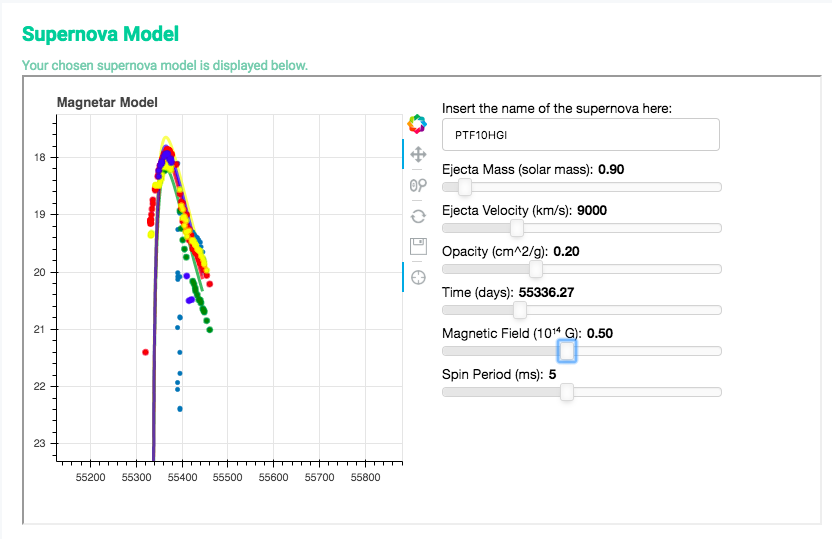
\includegraphics[scale=0.65,angle=0]{modeled.png}
\caption{Our web application fitting supernova PTF10hgi. \label{fig:1}}
\end{center}
\end{figure}

\acknowledgments

The authors are grateful to S. Gomez for helpful discussions throughout this work to and to J. Guillochon for help connecting to the OSC. LB and SG were participants in the Science Research Mentoring Program at the Center for Astrophysics \textbar{} Harvard \& Smithsonian \citep{2018arXiv180908078G}. Support for this program is provided by the National Science Foundation under award AST-1602595, City of Cambridge, the John G. Wolbach Library, Cambridge Rotary, and generous individuals. VAV is supported by a Ford Foundation Dissertation Fellowship.

\bibliography{mybib}

\end{document}
